\section{The Importance of Expert Knowledge in Survival Analysis}

While data-driven machine learning approaches to survival analysis offer tremendous potential \parencite{katzman2018,lee2018}, purely algorithmic methods may miss critical domain insights that are well-established in clinical research and practice \parencite{radfar2022,rudin2022}. This chapter explores how incorporating expert knowledge into survival models creates more robust, interpretable, and trustworthy predictions, particularly in high-stakes medical applications \parencite{kuo2020,ghassemi2022,karimi2021}.

\begin{notebox}[title=Chapter Overview]
This chapter covers:
\begin{itemize}
    \item Why expert knowledge is essential in survival analysis
    \item Types of domain expertise relevant to survival modeling
    \item Techniques for formalizing qualitative knowledge
    \item Parameter and feature-level constraint methods
    \item Neural architectures guided by expert knowledge
    \item Regularization and distillation approaches
    \item Case studies of expert-enhanced survival models
    \item Evaluation methods and future research directions
\end{itemize}
\end{notebox}

\section{Why Expert Knowledge Matters in Survival Analysis}

The integration of expert knowledge into survival analysis addresses several fundamental limitations of purely data-driven approaches.

\subsection{Limitations of Data-Only Approaches}

Despite advances in machine learning, survival models trained solely on available data face significant challenges:

\begin{itemize}
    \item \textbf{Limited training data:} Many survival datasets are small, especially for rare diseases or specific patient subgroups
    \item \textbf{Censoring creates fundamental uncertainties:} Right-censored observations provide incomplete information that may be supplemented by domain knowledge
    \item \textbf{Distribution shifts between populations:} Models trained on one population may not generalize well to others without incorporating expert understanding of underlying biology
    \item \textbf{Causal mechanisms vs. statistical correlations:} Statistical patterns may not reflect causal mechanisms understood by domain experts
    \item \textbf{Scientific understanding beyond observed patterns:} Decades of clinical research have established relationships that may not be apparent in limited datasets
\end{itemize}

\begin{figure}[htbp]
    \centering
    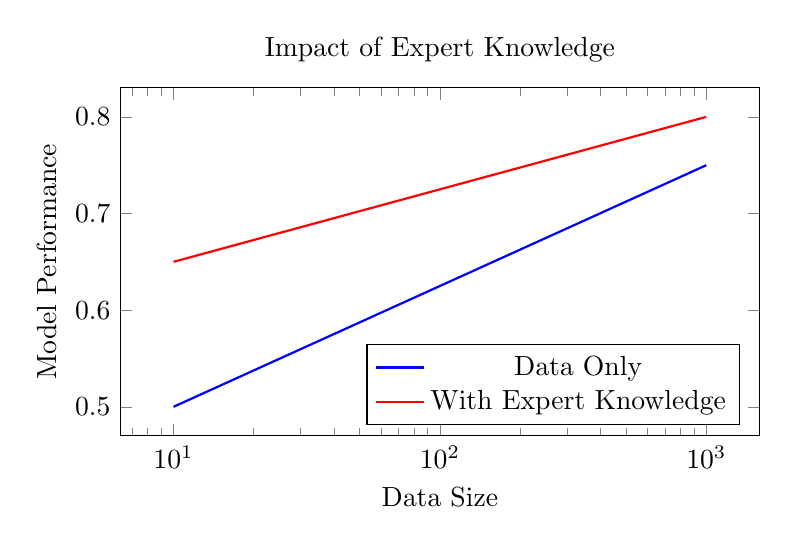
\begin{tikzpicture}
        \begin{axis}[
            width=0.8\textwidth,
            height=6cm,
            xlabel={Data Size},
            ylabel={Model Performance},
            title={Impact of Expert Knowledge},
            legend pos=south east,
            domain=10:1000,
            samples=100,
            xmode=log,
          ]
          % Data-only model
          \addplot[blue, thick] {0.5 + 0.25*ln(x/10)/ln(1000/10)};
          % Expert-guided model
          \addplot[red, thick] {0.65 + 0.15*ln(x/10)/ln(1000/10)};
          \legend{Data Only, With Expert Knowledge}
        \end{axis}
    \end{tikzpicture}
    \caption{The performance gap between data-only and expert-guided models. Expert knowledge provides the greatest benefit with smaller datasets but continues to improve performance even as data size increases.}
    \label{fig:expert-knowledge-impact}
\end{figure}

\subsection{The Gap Between Data and Understanding}

Medical knowledge represents a vast accumulation of understanding that cannot be fully captured in any single dataset:

\begin{itemize}
    \item \textbf{Observational vs. mechanistic understanding:} Statistical correlations may identify patterns, but experts understand the underlying biological mechanisms
    \item \textbf{Rare but important scenarios:} Experts have knowledge about rare conditions or edge cases that may be underrepresented in available data
    \item \textbf{Longitudinal progression:} Clinical expertise includes understanding of disease trajectories that may extend beyond available follow-up periods
    \item \textbf{Treatment effect modifiers:} Domain knowledge about which factors influence treatment efficacy may not be apparent from limited trial data
    \item \textbf{Physiological constraints:} Biological systems operate within constraints that should be reflected in predictive models
\end{itemize}

\begin{examplebox}[title=Expert Knowledge in Cancer Prognosis]
In cancer modeling, expert oncologists understand that:
\begin{itemize}
    \item Hazard functions typically increase over time as tumors grow (suggesting Weibull distributions with shape parameter $> 1$)
    \item Risk factors like tumor size, grade, and certain biomarkers have monotonically increasing effects on risk
    \item Different cancer subtypes have distinct survival patterns that may require different parameter ranges
    \item Treatment effects often follow specific temporal patterns (e.g., initial benefit followed by potential resistance)
    \item Competing risks (cancer death vs. other causes) have specific dependency structures
\end{itemize}
This knowledge can be formalized as constraints, priors, or architectural guidance for survival models.
\end{examplebox}

\section{Types of Expert Knowledge in Survival Analysis}

Domain expertise relevant to survival analysis comes in several forms, each informing different aspects of model development.

\subsection{Forms of Domain Expertise}

\subsubsection{Distributional Knowledge}

Experts often have insights about the overall patterns of event timing:

\begin{itemize}
    \item \textbf{Shape of hazard functions:} Understanding whether risk increases, decreases, or follows more complex patterns over time
    \item \textbf{Expected survival patterns:} Knowledge of typical survival curves for specific conditions
    \item \textbf{Parametric families for events:} Insights about which distributions best model certain diseases (e.g., Weibull for cancer progression)
    \item \textbf{Common censoring mechanisms:} Understanding the patterns and reasons for censoring in specific domains
\end{itemize}

\subsubsection{Feature Relationships}

Clinical expertise includes knowledge about risk factors and their effects:

\begin{itemize}
    \item \textbf{Known risk factors:} Established predictors for specific outcomes
    \item \textbf{Effect directions:} Whether factors increase or decrease risk
    \item \textbf{Interaction effects:} How factors modify each other's impact on risk
    \item \textbf{Non-linear relationships:} Knowledge of threshold effects, U-shaped relationships, or plateaus
    \item \textbf{Effect magnitudes:} Relative importance of different predictors
\end{itemize}

\subsubsection{Temporal Patterns}

Time-dependent aspects of risk are particularly relevant to survival analysis:

\begin{itemize}
    \item \textbf{Expected changes over time:} How risk evolves with disease duration
    \item \textbf{Time-varying effects:} Factors whose influence changes over the follow-up period
    \item \textbf{Critical time periods:} Windows of particularly high or low risk
    \item \textbf{Treatment timing effects:} How intervention timing influences outcomes
\end{itemize}

\subsubsection{Event Dependencies}

In multi-event settings, experts understand relationships between different outcomes:

\begin{itemize}
    \item \textbf{Relationships between competing risks:} How different event types relate to each other
    \item \textbf{Causal connections:} When one event directly influences the risk of another
    \item \textbf{Conditional dependencies:} How risk relationships change given certain events or treatments
    \item \textbf{Sequential patterns:} Typical progression paths through multiple events
\end{itemize}

\subsubsection{Population Heterogeneity}

Experts recognize distinct patterns across patient subgroups:

\begin{itemize}
    \item \textbf{Subgroup differences:} How risk profiles differ across patient segments
    \item \textbf{Patient stratification criteria:} Factors that define meaningful subgroups
    \item \textbf{Treatment effect modifiers:} Characteristics that influence treatment response
    \item \textbf{Age and demographic effects:} How risk varies across demographic factors
\end{itemize}

\subsubsection{Biological Mechanisms}

Understanding of underlying biological processes informs risk patterns:

\begin{itemize}
    \item \textbf{Disease progression patterns:} Stages and mechanisms of disease evolution
    \item \textbf{Physiological constraints:} Biological limits that constrain possible outcomes
    \item \textbf{Treatment response dynamics:} Mechanisms of therapeutic effect and resistance
    \item \textbf{Compensatory systems:} How biological systems adapt to changes
\end{itemize}

\subsection{Sources of Expert Knowledge}

Domain expertise can be derived from various sources:

\begin{itemize}
    \item \textbf{Clinical practice guidelines:} Consensus recommendations from professional societies
    \item \textbf{Published medical literature:} Peer-reviewed research and meta-analyses
    \item \textbf{Established risk scores and nomograms:} Validated clinical prediction tools
    \item \textbf{Direct clinician consultations:} Interviews with subject matter experts
    \item \textbf{Consensus panel recommendations:} Formalized expert opinions
    \item \textbf{Mechanistic models from biology/physiology:} Mathematical models of underlying processes
    \item \textbf{Previous clinical trials and meta-analyses:} Aggregated evidence from controlled studies
    \item \textbf{Disease registries and historical data:} Long-term observational records
\end{itemize}

\begin{figure}[htbp]
    \centering
    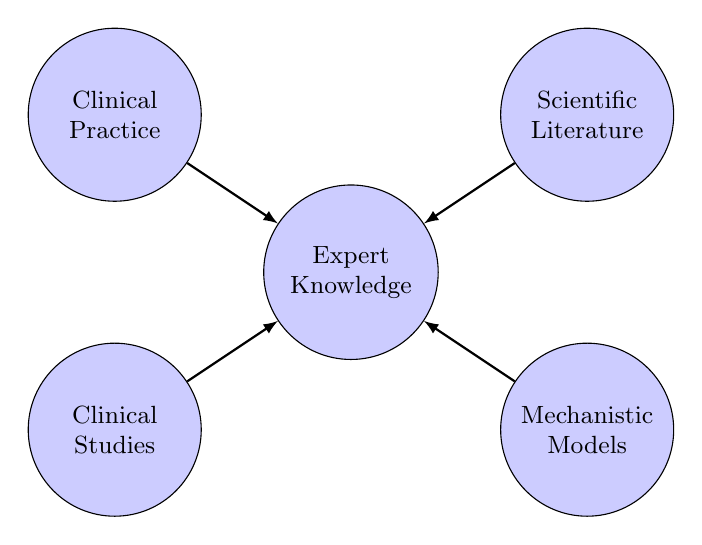
\begin{tikzpicture}[
        concept/.style={circle, draw=black, fill=blue!20,
          minimum size=2cm, text width=1.8cm,
          align=center, font=\small},
        connection/.style={->, >=latex, thick}
      ]
      \node[concept] (center) at (0,0) {Expert Knowledge};

      \node[concept] (clinical) at (-3,2) {Clinical Practice};
      \node[concept] (literature) at (3,2) {Scientific Literature};
      \node[concept] (studies) at (-3,-2) {Clinical Studies};
      \node[concept] (models) at (3,-2) {Mechanistic Models};

      \draw[connection] (clinical) -- (center);
      \draw[connection] (literature) -- (center);
      \draw[connection] (studies) -- (center);
      \draw[connection] (models) -- (center);
    \end{tikzpicture}
    \caption{Sources of expert knowledge for integration into survival models. Multiple sources contribute to a comprehensive understanding that can guide model development.}
    \label{fig:expert-knowledge-sources}
\end{figure}

\section{Challenges in Knowledge Integration}

Incorporating expert knowledge into statistical models presents several challenges that must be addressed for successful implementation.

\subsection{Formalization Challenges}

Converting qualitative expertise into quantitative model constraints is a fundamental challenge:

\begin{itemize}
    \item \textbf{Converting qualitative expertise to quantitative constraints:} Experts often express knowledge in qualitative terms that must be translated into mathematical formulations
    \item \textbf{Representing uncertainty in expert knowledge:} Experts have varying degrees of confidence in different aspects of their knowledge
    \item \textbf{Handling conflicting expert opinions:} Different experts may have contradictory views on certain aspects of disease progression
    \item \textbf{Translating clinical language to mathematical formulations:} Bridging the gap between medical terminology and statistical concepts
    \item \textbf{Capturing context-dependent knowledge:} Expert insights that apply only in specific situations
\end{itemize}

\subsection{Integration Challenges}

Balancing expert knowledge with data-driven learning presents additional challenges:

\begin{itemize}
    \item \textbf{Balancing data evidence vs. prior knowledge:} Determining how strongly to weight expert priors relative to observed data
    \item \textbf{Incorporating knowledge without overly restricting the model:} Allowing flexibility to learn patterns not anticipated by experts
    \item \textbf{Maintaining computational tractability:} Some constraints may significantly increase model complexity
    \item \textbf{Adapting knowledge strength to data size:} Reducing the influence of priors as data volume increases
    \item \textbf{Updating knowledge based on new evidence:} Incorporating feedback loops to refine expert knowledge
\end{itemize}

\subsection{Validation Challenges}

Evaluating the impact of expert knowledge integration introduces methodological challenges:

\begin{itemize}
    \item \textbf{Measuring the value added by expert knowledge:} Quantifying improvement over purely data-driven approaches
    \item \textbf{Testing if knowledge incorporation improves generalization:} Verifying better performance on new populations
    \item \textbf{Detecting when expertise conflicts with data evidence:} Identifying situations where expert knowledge may be misleading
    \item \textbf{Determining when to override expert priors:} Criteria for letting data outweigh prior knowledge
    \item \textbf{Developing fairness metrics for knowledge-guided models:} Ensuring that expert knowledge doesn't introduce or amplify biases
\end{itemize}

\section{Knowledge Formalization Techniques}

Before expert knowledge can be incorporated into models, it must be formalized through structured processes.

\subsection{Elicitation Methods}

Several approaches can systematically capture expert knowledge:

\begin{itemize}
    \item \textbf{Structured interviews with domain experts:} One-on-one discussions following established protocols
    \item \textbf{Survey techniques with confidence ratings:} Questionnaires that capture both judgments and confidence levels
    \item \textbf{Delphi method for consensus building:} Iterative anonymous feedback process to reach expert consensus
    \item \textbf{Literature review and meta-analysis:} Systematic synthesis of published evidence
    \item \textbf{Analysis of existing clinical models:} Reverse-engineering established prediction tools
    \item \textbf{Feature importance rankings:} Expert prioritization of predictive factors
    \item \textbf{Qualitative to quantitative mapping frameworks:} Structured conversion of verbal descriptions to numeric constraints
\end{itemize}

\begin{figure}[htbp]
    \centering
    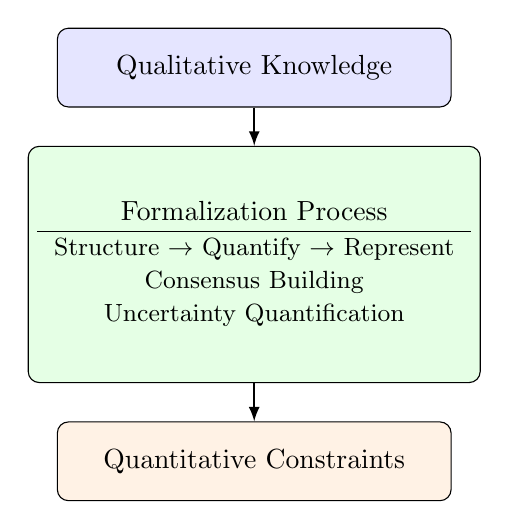
\begin{tikzpicture}
        \node[draw, rounded corners, minimum width=5cm, minimum height=1cm, fill=blue!10] (qualitative) at (0,0) {Qualitative Knowledge};

        \node[draw, rounded corners, minimum width=5cm, minimum height=3cm, fill=green!10] (formalization) at (0,-2.5) {
            \begin{tabular}{c}
                Formalization Process \\
                \hline
                \small{Structure} $\rightarrow$ \small{Quantify} $\rightarrow$ \small{Represent} \\
                \small{Consensus Building} \\
                \small{Uncertainty Quantification}
            \end{tabular}
        };

        \node[draw, rounded corners, minimum width=5cm, minimum height=1cm, fill=orange!10] (quantitative) at (0,-5) {Quantitative Constraints};

        \draw[-latex, thick] (qualitative) -- (formalization);
        \draw[-latex, thick] (formalization) -- (quantitative);
    \end{tikzpicture}
    \caption{The knowledge formalization process converts qualitative expert insights into quantitative model constraints through structured elicitation and representation techniques.}
    \label{fig:knowledge-formalization}
\end{figure}

\subsection{Bayesian Frameworks}

Bayesian statistics provides a natural framework for incorporating expert knowledge:

\begin{itemize}
    \item \textbf{Prior distribution elicitation:} Capturing expert beliefs as probability distributions over parameters
    \item \textbf{Hierarchical priors:} Structured prior frameworks that allow for uncertainty in expert knowledge
    \item \textbf{Equivalent sample size determination:} Quantifying the strength of prior knowledge relative to observed data
    \item \textbf{Prior predictive checks:} Verifying that prior distributions lead to reasonable predictions
\end{itemize}

\section{Parameter Constraints in Survival Models}

One of the most direct approaches to incorporating expert knowledge is through constraints on model parameters, particularly those governing the shape of hazard functions.

\subsection{Disease-Specific Shape Parameters}

For parametric survival models like the Weibull distribution, experts can provide guidance on appropriate parameter ranges:

\begin{equationbox}[title=Weibull Distribution Parameters]
The Weibull distribution has two key parameters:
\begin{itemize}
    \item Shape parameter $\alpha$: Controls whether hazard increases ($\alpha > 1$), decreases ($\alpha < 1$), or remains constant ($\alpha = 1$) over time
    \item Scale parameter $\lambda$: Related to the median survival time
\end{itemize}

Expert knowledge can constrain these parameters based on disease characteristics:
\begin{align}
    h(t) = \frac{\alpha}{\lambda}\left(\frac{t}{\lambda}\right)^{\alpha-1}
\end{align}
\end{equationbox}

\begin{examplebox}[title=Disease-Specific Shape Constraints]
Experts can provide guidance on shape parameters for different conditions:

\begin{itemize}
    \item \textbf{Cancer progression:} $\alpha > 1$ (increasing hazard)
    \begin{itemize}
        \item Tumor growth accelerates damage over time
        \item Metastatic spread increases with disease duration
        \item Example: $\alpha \in [1.2, 2.5]$ for breast cancer
    \end{itemize}

    \item \textbf{Infectious disease:} $\alpha < 1$ (decreasing hazard)
    \begin{itemize}
        \item Highest risk immediately after exposure/infection
        \item Immune response decreases hazard over time
        \item Example: $\alpha \in [0.5, 0.9]$ for post-surgical infection
    \end{itemize}

    \item \textbf{Chronic conditions:} $\alpha \approx 1$ (constant hazard)
    \begin{itemize}
        \item Ongoing risk remains relatively stable
        \item Random event occurrence pattern
        \item Example: $\alpha \in [0.9, 1.1]$ for chronic heart failure
    \end{itemize}
\end{itemize}
\end{examplebox}

\subsection{Implementation Approaches for Parameter Constraints}

Several techniques can enforce expert-defined parameter constraints:

\begin{itemize}
    \item \textbf{Parameter bounding:} Ensure parameters remain within valid ranges using transformations
    \begin{align}
        \alpha = \alpha_{min} + \text{softplus}(w)
    \end{align}

    \item \textbf{Informative priors:} Use probability distributions that encode expert knowledge
    \begin{align}
        \alpha \sim \text{Gamma}(a, b)
    \end{align}

    \item \textbf{Penalty terms:} Add regularization that penalizes deviation from expert expectations
    \begin{align}
        \mathcal{L}_{penalty} = \lambda(\alpha - \alpha_{prior})^2
    \end{align}

    \item \textbf{Constrained activation:} Use bounded activation functions to enforce parameter limits
    \begin{align}
        \alpha = \alpha_{min} + (\alpha_{max} - \alpha_{min})\sigma(w)
    \end{align}
    where $\sigma$ is the sigmoid function
\end{itemize}

\begin{figure}[htbp]
    \centering
    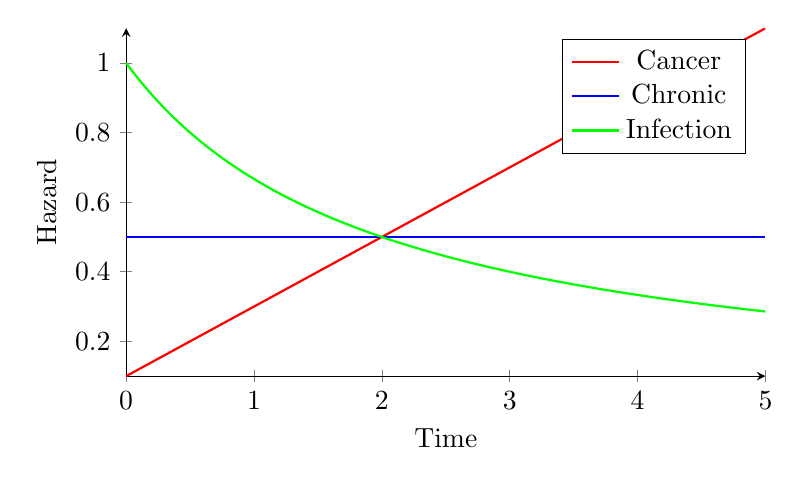
\begin{tikzpicture}
        \begin{axis}[
            width=0.8\textwidth,
            height=6cm,
            xlabel={Time},
            ylabel={Hazard},
            axis lines=left,
            domain=0:5,
            samples=100,
            legend pos=north east,
          ]
          % Cancer progression (increasing hazard)
          \addplot[red, thick] {0.2*x + 0.1};
          % Chronic disease (constant hazard)
          \addplot[blue, thick] {0.5};
          % Infectious disease (decreasing hazard)
          \addplot[green, thick] {1/(1 + 0.5*x)};
          \legend{Cancer, Chronic, Infection}
        \end{axis}
    \end{tikzpicture}
    \caption{Expert-guided hazard shapes for different disease types. Cancer typically shows increasing hazard (red), chronic conditions often have constant hazard (blue), and infectious complications frequently show decreasing hazard over time (green).}
    \label{fig:expert-hazard-shapes}
\end{figure}

\section{Feature-Level Expert Constraints}

Beyond distributional parameters, expert knowledge can inform how individual features relate to survival outcomes.

\subsection{Knowledge About Risk Factors}

Experts typically have well-established understanding of how specific variables influence risk:

\begin{itemize}
    \item \textbf{Sign constraints:} Force coefficients to have expert-expected signs
    \begin{itemize}
        \item Example: Age coefficient must be positive for most diseases
        \item Implementation: $\beta_{age} = \text{softplus}(w)$
    \end{itemize}

    \item \textbf{Relative importance:} Constrain relative magnitudes of feature effects
    \begin{itemize}
        \item Example: Smoking impact > BMI impact for lung cancer
        \item Implementation: $|\beta_{smoking}| > |\beta_{BMI}|$
    \end{itemize}

    \item \textbf{Feature grouping:} Related features should have similar effects
    \begin{itemize}
        \item Example: Various cholesterol measures
        \item Implementation: Group lasso or similarity penalties
    \end{itemize}
\end{itemize}

\subsection{Monotonicity Constraints}

Many risk factors are known to have consistently increasing or decreasing effects:

\begin{itemize}
    \item \textbf{Monotonic feature effects:} Enforce consistently directional relationships
    \begin{itemize}
        \item Risk monotonically increases with age
        \item Blood pressure has threshold effects
        \item Implementation: constrained neural networks
    \end{itemize}

    \item \textbf{Methods for monotonicity:}
    \begin{itemize}
        \item Positive-weight-only networks
        \item Monotonic spline transformations
        \item Architectural constraints in layers
        \item Gradient penalties during training
    \end{itemize}
\end{itemize}

\begin{figure}[htbp]
    \centering
    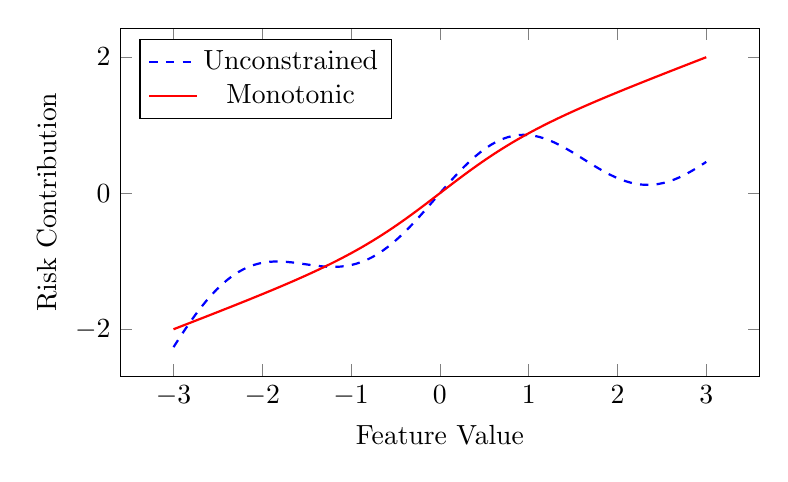
\begin{tikzpicture}
        \begin{axis}[
            width=0.8\textwidth,
            height=6cm,
            xlabel={Feature Value},
            ylabel={Risk Contribution},
            domain=-3:3,
            samples=100,
            legend pos=north west,
          ]
          % Unconstrained function
          \addplot[blue, dashed, thick] {0.5*x - 0.1*x^2 + 0.5*sin(deg(2*x))};
          % Monotonically constrained function
          \addplot[red, thick] {0.5*x + 0.5*tanh(x)};
          \legend{Unconstrained, Monotonic}
        \end{axis}
    \end{tikzpicture}
    \caption{Comparison of unconstrained (blue) and monotonically constrained (red) feature effects. The unconstrained function can learn arbitrary patterns, while the monotonic constraint ensures the relationship consistently increases with the feature value, aligning with expert knowledge.}
    \label{fig:monotonic-constraints}
\end{figure}

\section{Expert-Guided Neural Architectures}

The architecture of neural survival models can be designed to incorporate expert knowledge directly into the model structure.

\subsection{Structure Constraints for Networks}

Network architecture can reflect expert understanding of feature importance and relationships:

\begin{itemize}
    \item \textbf{Feature importance constraints:}
    \begin{itemize}
        \item Force known risk factors to have high weights
        \item Regularize less well-understood features more heavily
        \item $\mathcal{L}_{reg} = \sum_i w_i |\theta_i|$ where $w_i$ is feature-specific regularization
    \end{itemize}

    \item \textbf{Attention mechanisms:}
    \begin{itemize}
        \item Guide attention to focus on important features
        \item Prior attention masks from domain knowledge
        \item Semi-supervised attention learning
    \end{itemize}

    \item \textbf{Dependency structures:}
    \begin{itemize}
        \item Expert-defined event dependency matrix $D_{ij}$ between risks
        \item Encode in the MENSA dependency layer architecture
        \item $\pi_{jk}(x) = g(W_j \cdot \phi(x) + \sum_i D_{ij} \cdot W_i \cdot \phi(x))$
    \end{itemize}
\end{itemize}

\subsection{Dedicated Architecture for Expert Constraints}

Custom network architectures can be designed specifically to incorporate expert knowledge at multiple levels:

\begin{figure}[htbp]
    \centering
    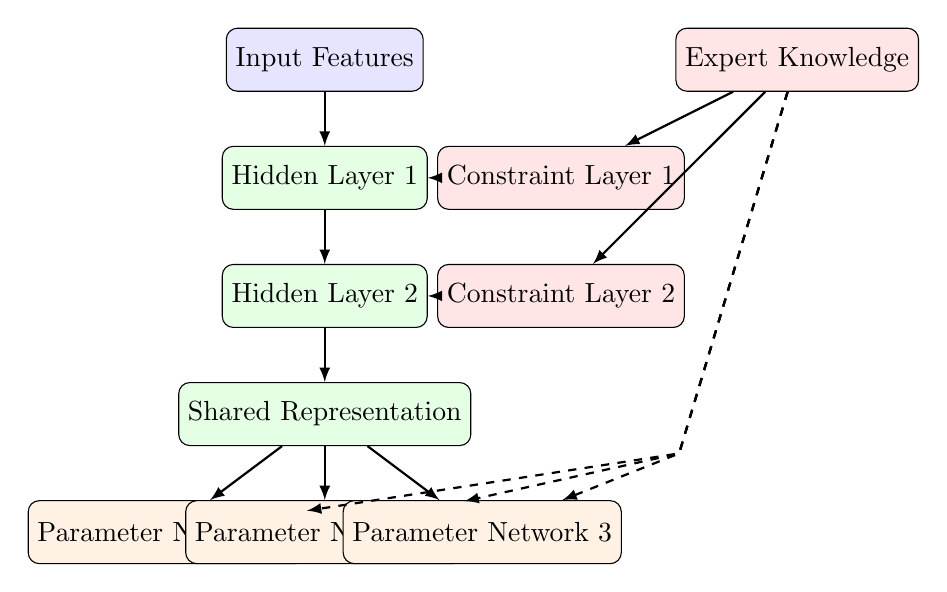
\begin{tikzpicture}[
        box/.style={rectangle, draw, rounded corners, minimum width=2.5cm, minimum height=0.8cm},
        arrow/.style={->, >=latex, thick}
      ]
      % Input layer
      \node[box, fill=blue!10] (input) at (0,0) {Input Features};

      % Expert knowledge
      \node[box, fill=red!10] (expert) at (6,0) {Expert Knowledge};

      % Hidden layers with expert influence
      \node[box, fill=green!10] (h1) at (0,-1.5) {Hidden Layer 1};
      \node[box, fill=red!10] (c1) at (3,-1.5) {Constraint Layer 1};

      \node[box, fill=green!10] (h2) at (0,-3) {Hidden Layer 2};
      \node[box, fill=red!10] (c2) at (3,-3) {Constraint Layer 2};

      \node[box, fill=green!10] (shared) at (0,-4.5) {Shared Representation};

      % Output layers
      \node[box, fill=orange!10] (param1) at (-2,-6) {Parameter Network 1};
      \node[box, fill=orange!10] (param2) at (0,-6) {Parameter Network 2};
      \node[box, fill=orange!10] (param3) at (2,-6) {Parameter Network 3};

      % Connect everything
      \draw[arrow] (input) -- (h1);
      \draw[arrow] (h1) -- (h2);
      \draw[arrow] (h2) -- (shared);

      \draw[arrow] (shared) -- (param1);
      \draw[arrow] (shared) -- (param2);
      \draw[arrow] (shared) -- (param3);

      % Expert knowledge connections
      \draw[arrow] (expert) -- (c1);
      \draw[arrow] (expert) -- (c2);
      \draw[arrow, dashed] (expert) -- (4.5,-5) -- (param1);
      \draw[arrow, dashed] (expert) -- (4.5,-5) -- (param2);
      \draw[arrow, dashed] (expert) -- (4.5,-5) -- (param3);

      % Constraint connections
      \draw[arrow] (c1) -- (h1);
      \draw[arrow] (c2) -- (h2);
    \end{tikzpicture}
    \caption{Architecture for expert knowledge integration into a neural survival model. Expert knowledge influences the network at multiple levels: constraining intermediate representations, guiding feature learning, and directly shaping distribution parameters.}
    \label{fig:expert-architecture}
\end{figure}

This architecture incorporates expert knowledge at multiple levels:
\begin{itemize}
    \item Constraint layers directly modify hidden representations based on expert knowledge
    \item Direct connections to parameter networks enforce constraints on distribution parameters
    \item The entire architecture reflects the causal structure understood by domain experts
\end{itemize}

\section{Expert Knowledge as Regularization}

Rather than strictly constraining the model, expert knowledge can be incorporated as regularization that guides learning while still allowing data to drive the primary optimization.

\subsection{Training with Expert Priors}

Expert knowledge can be formalized as prior distributions and incorporated into the objective function:

\begin{equationbox}[title=Expert-Guided Regularization]
Prior distribution on parameters given expert knowledge:
\begin{align}
    p(\theta | \text{expert}) \propto \exp(-\lambda R(\theta, \text{expert}))
\end{align}

Regularized log-likelihood:
\begin{align}
    \mathcal{L}_{reg} = \mathcal{L}_{data} + \lambda R(\theta, \text{expert})
\end{align}

where $\lambda$ controls the strength of the expert prior relative to the data likelihood.
\end{equationbox}

\subsection{Common Regularization Forms}

Several forms of regularization can encode different types of expert knowledge:

\begin{itemize}
    \item \textbf{Parameter-targeted:} Regularize model parameters directly
    \begin{align}
        R(\theta, \text{expert}) = \|\theta - \theta_{expert}\|^2
    \end{align}

    \item \textbf{Output-targeted:} Regularize model predictions toward expert expectations
    \begin{align}
        R(\theta, \text{expert}) = \|f_\theta(x) - f_{expert}(x)\|^2
    \end{align}

    \item \textbf{Structure-targeted:} Regularize intermediate representations to align with expert understanding
    \begin{align}
        R(\theta, \text{expert}) = \|g_\theta(x) - g_{expert}(x)\|^2
    \end{align}
    where $g_\theta$ represents intermediate representations

    \item \textbf{Adaptive weighting:} Adjust regularization strength based on data size
    \begin{align}
        \lambda = \lambda_0 \cdot \frac{n_0}{n_0 + n}
    \end{align}
    where $n_0$ represents the "equivalent sample size" of expert knowledge
\end{itemize}

\section{Knowledge Distillation from Expert Models}

Another approach to incorporating expert knowledge is through knowledge distillation from simpler, more interpretable models developed based on expert understanding.

\subsection{Model Distillation Process}

Knowledge distillation transfers insights from expert-developed models to more flexible neural models:

\begin{itemize}
    \item \textbf{Expert models as teachers:}
    \begin{itemize}
        \item Traditional survival models built by experts
        \item Disease-specific simplified models
        \item Clinical risk scores and nomograms
        \item Established causal models
    \end{itemize}

    \item \textbf{Distillation process:}
    \begin{align}
        \mathcal{L}_{distill} = \alpha \mathcal{L}_{data} + (1-\alpha) \mathcal{L}_{expert}
    \end{align}

    \item \textbf{Distillation techniques:}
    \begin{itemize}
        \item Prediction matching: $\|f_\theta(x) - f_{expert}(x)\|^2$
        \item Feature attention matching
        \item Gradient similarity enforcement
        \item Representation alignment
    \end{itemize}
\end{itemize}

\begin{figure}[htbp]
    \centering
    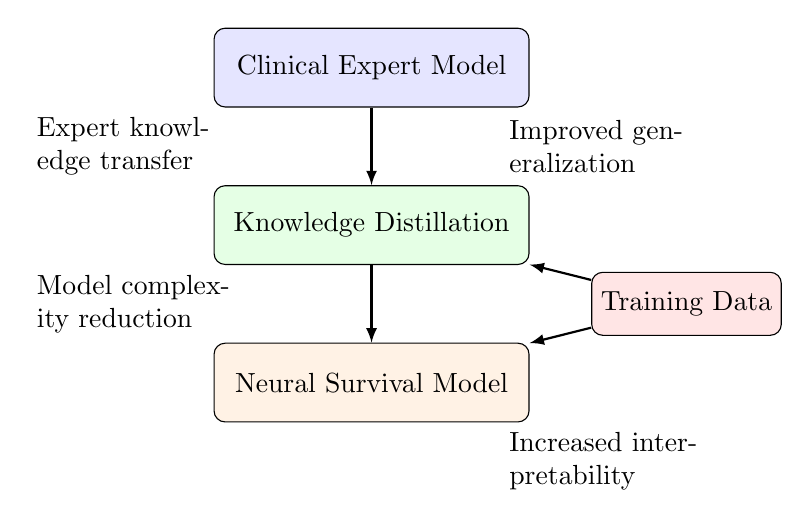
\begin{tikzpicture}
        \node[rectangle, rounded corners, draw, fill=blue!10, minimum width=4cm, minimum height=1cm] (clinicalmodel) at (0,0) {Clinical Expert Model};

        \node[rectangle, rounded corners, draw, fill=green!10, minimum width=4cm, minimum height=1cm] (distillation) at (0,-2) {Knowledge Distillation};

        \node[rectangle, rounded corners, draw, fill=orange!10, minimum width=4cm, minimum height=1cm] (neuralmodel) at (0,-4) {Neural Survival Model};

        \draw[-latex, thick] (clinicalmodel) -- (distillation);
        \draw[-latex, thick] (distillation) -- (neuralmodel);

        % Add data arrow
        \node[rectangle, rounded corners, draw, fill=red!10, minimum width=2cm, minimum height=0.8cm] (data) at (4,-3) {Training Data};
        \draw[-latex, thick] (data) -- (distillation);
        \draw[-latex, thick] (data) -- (neuralmodel);

        % Add benefits
        \node[align=left, text width=2.5cm] at (-3,-1) {Expert knowledge transfer};
        \node[align=left, text width=2.5cm] at (-3,-3) {Model complexity reduction};
        \node[align=left, text width=2.5cm] at (3,-1) {Improved generalization};
        \node[align=left, text width=2.5cm] at (3,-5) {Increased interpretability};
    \end{tikzpicture}
    \caption{Knowledge distillation process. A simple, expert-developed clinical model serves as a teacher for a more complex neural survival model, transferring domain knowledge while maintaining the flexibility of deep learning approaches.}
    \label{fig:knowledge-distillation}
\end{figure}

\section{Expert-Guided Ensemble Methods}

Ensemble methods offer another approach to combine the benefits of expert knowledge and data-driven learning.

\subsection{Combining Models with Expert Weights}

Expert knowledge can guide the combination of multiple model types:

\begin{itemize}
    \item \textbf{Expert-weighted ensemble:}
    \begin{align}
        f_{ensemble}(x) = \sum_{m=1}^M w_m f_m(x)
    \end{align}
    where $w_m$ are expert-defined model weights

    \item \textbf{Model class weighting:}
    \begin{itemize}
        \item Combine parametric, ML, and mechanistic models
        \item Weights based on expert confidence in model types
        \item Example: 0.5 × Cox + 0.3 × Neural + 0.2 × Mechanistic
    \end{itemize}

    \item \textbf{Context-dependent weighting:}
    \begin{itemize}
        \item Expert rules for when to trust which model
        \item Different weights for different patient subgroups
        \item Gating network trained with expert guidance
    \end{itemize}
\end{itemize}

\section{Case Study: Expert-Guided MENSA for Cardiovascular Disease}

To illustrate the practical application of expert knowledge integration, we present a case study of an expert-guided Multi-Event Neural Survival Analysis (MENSA) model for cardiovascular disease prediction.

\subsection{Problem: Complex Dependencies in Cardiovascular Disease}

Cardiovascular disease (CVD) involves multiple interrelated events with complex dependencies:

\begin{itemize}
    \item Multiple competing events: heart attack, stroke, heart failure
    \item These events have known physiological dependencies
    \item Traditional models treat them as independent
    \item Limited data for some combinations of events
    \item Patient subgroups have distinct risk profiles
\end{itemize}

\subsection{Expert Knowledge Integration}

Cardiologists provided structured knowledge to enhance the MENSA model:

\begin{itemize}
    \item \textbf{Event dependency structure:}
    Cardiologists defined a dependency matrix between events
    \begin{align}
        D =
        \begin{pmatrix}
            1.0 & 0.7 & 0.5 \\
            0.7 & 1.0 & 0.3 \\
            0.5 & 0.3 & 1.0
        \end{pmatrix}
        \quad
        \begin{array}{c}
            \text{heart attack} \\
            \text{stroke} \\
            \text{heart failure}
        \end{array}
    \end{align}

    \item \textbf{Feature importance constraints:} 
    Based on established Framingham risk score
    \begin{itemize}
        \item Age, blood pressure, cholesterol given stronger weights
        \item Novel biomarkers allowed more flexibility
    \end{itemize}

    \item \textbf{Parameter constraints:} 
    Age-dependent hazard shapes for each event
\end{itemize}

\subsection{Results and Evaluation}

The expert-guided model showed significant improvements over standard MENSA:

\begin{center}
    \begin{tabular}{l|cc}
        \hline
        Model & C-index & Calibration \\
        \hline
        Standard MENSA & 0.71 & 0.15 \\
        Expert-guided & \textbf{0.73} & \textbf{0.08} \\
        \hline
    \end{tabular}
\end{center}

Key benefits included:
\begin{itemize}
    \item Better performance with limited data
    \item Significantly improved calibration
    \item More realistic risk interdependencies
    \item Enhanced clinician trust and adoption
    \item Better generalization to new populations
\end{itemize}

\begin{figure}[htbp]
    \centering
    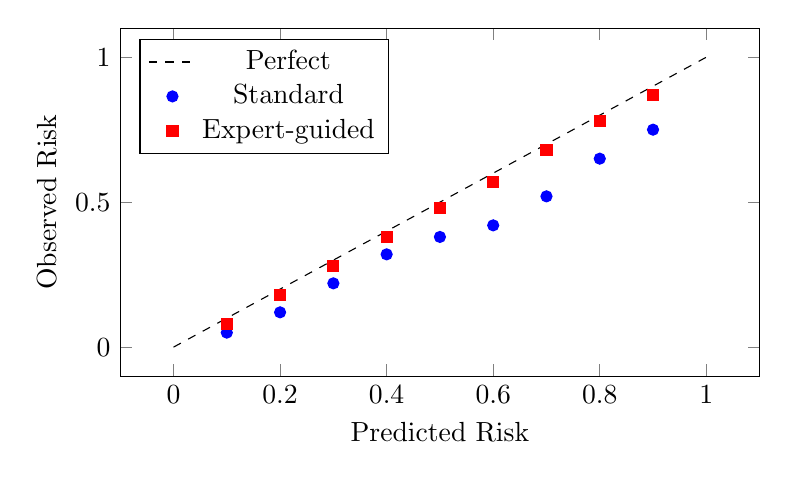
\begin{tikzpicture}
        \begin{axis}[
            width=0.8\textwidth,
            height=6cm,
            xlabel={Predicted Risk},
            ylabel={Observed Risk},
            domain=0:1,
            samples=100,
            legend pos=north west,
          ]
          % Perfect calibration
          \addplot[black, dashed] {x};
          % Standard model
          \addplot[blue, mark=*, only marks] coordinates {
            (0.1, 0.05) (0.2, 0.12) (0.3, 0.22)
            (0.4, 0.32) (0.5, 0.38) (0.6, 0.42)
            (0.7, 0.52) (0.8, 0.65) (0.9, 0.75)
          };
          % Expert-guided model
          \addplot[red, mark=square*, only marks] coordinates {
            (0.1, 0.08) (0.2, 0.18) (0.3, 0.28)
            (0.4, 0.38) (0.5, 0.48) (0.6, 0.57)
            (0.7, 0.68) (0.8, 0.78) (0.9, 0.87)
          };
          \legend{Perfect, Standard, Expert-guided}
        \end{axis}
    \end{tikzpicture}
    \caption{Calibration plot comparing standard MENSA (blue) and expert-guided MENSA (red). The expert-guided model shows improved alignment with the perfect calibration line (dashed), indicating better agreement between predicted and observed risks.}
    \label{fig:calibration-comparison}
\end{figure}

\section{Integrating Expert Knowledge in the Workflow}

Expert knowledge integration should be a systematic process throughout the model development lifecycle.

\begin{figure}[htbp]
    \centering
    \begin{tikzpicture}[
        node distance=1.5cm,
        box/.style={rectangle, rounded corners, draw, minimum width=3cm, minimum height=0.8cm}
      ]
      % Expert knowledge side
      \node[box, fill=blue!10] (expert) {Domain Expertise};
      \node[box, fill=blue!10, below=of expert] (formalization) {Knowledge Formalization};
      \node[box, fill=blue!10, below=of formalization] (constraints) {Constraints \& Priors};
      
      % Data side
      \node[box, fill=green!10, right=6cm of expert] (data) {Survival Data};
      \node[box, fill=green!10, below=of data] (preprocessing) {Preprocessing};
      \node[box, fill=green!10, below=of preprocessing] (features) {Feature Engineering};
      
      % Model side (center, bottom)
      \node[box, fill=orange!10, below=3cm of constraints, xshift=3cm] (architecture) {Model Architecture};
      \node[box, fill=orange!10, below=of architecture] (training) {Constrained Training};
      \node[box, fill=orange!10, below=of training] (evaluation) {Evaluation};
      
      % Connections from expert side
      \draw[-latex] (expert) -- (formalization);
      \draw[-latex] (formalization) -- (constraints);
      \draw[-latex] (constraints) -- node[left, align=right] {Shape\\constraints} (architecture);
      \draw[-latex] (constraints) -| node[above, align=center, near start] {Prior\\distributions} (training);
      
      % Connections from data side
      \draw[-latex] (data) -- (preprocessing);
      \draw[-latex] (preprocessing) -- (features);
      \draw[-latex] (features) -| (architecture);
      \draw[-latex] (features) -| (training);
      
      % Model flow
      \draw[-latex] (architecture) -- (training);
      \draw[-latex] (training) -- (evaluation);
      
      % Expert validation
      \draw[-latex] (evaluation) -- ++(0,-1) -| node[below, align=center, near end] {Validation against\\expert knowledge} (expert);
    \end{tikzpicture}
    \caption{Integrated workflow for expert knowledge in survival modeling. Expert knowledge and data flow in parallel through the modeling process, with expertise informing architecture design, parameter constraints, and training regularization.}
    \label{fig:expert-workflow}
\end{figure}

Key phases in this workflow include:
\begin{itemize}
    \item \textbf{Knowledge elicitation:} Systematic capture of domain expertise
    \item \textbf{Formalization:} Translation into mathematical constraints
    \item \textbf{Architecture design:} Incorporating expertise into model structure
    \item \textbf{Constrained training:} Parameter learning guided by expert priors
    \item \textbf{Evaluation:} Assessment against both data-driven and expert-defined metrics
    \item \textbf{Feedback loop:} Refinement of expert knowledge based on model performance
\end{itemize}

\section{Measuring the Impact of Expert Knowledge}

Rigorous evaluation is essential to quantify the value added by expert knowledge integration.

\subsection{Evaluation Approaches}

Several complementary approaches can assess the impact of expert knowledge:

\begin{itemize}
    \item \textbf{Ablation studies:}
    \begin{itemize}
        \item Compare with and without expert priors
        \item Vary strength of expert constraints
        \item Measure performance impact by constraint type
    \end{itemize}

    \item \textbf{Out-of-distribution testing:}
    \begin{itemize}
        \item Test on populations different from training
        \item Evaluate performance on rare subgroups
        \item Measure robustness to data shifts
    \end{itemize}

    \item \textbf{Expert evaluation:}
    \begin{itemize}
        \item Clinical review of model predictions
        \item Assessment of prediction explanations
        \item Trust and adoption metrics
    \end{itemize}
\end{itemize}

\section{Challenges and Future Research Directions}

While expert knowledge integration offers significant benefits, several challenges and open research questions remain.

\subsection{Current Limitations}

Expert knowledge integration faces several practical challenges:

\begin{itemize}
    \item Experts may disagree or have outdated knowledge
    \item Difficult to quantify confidence in expert opinions
    \item Overly strong priors may prevent learning from data
    \item Domain expertise may not transfer across populations
    \item Balancing expert knowledge with data-driven discovery
    \item Computational complexity of some constraint forms
\end{itemize}

\subsection{Future Research Directions}

Several promising research directions may address these challenges:

\begin{itemize}
    \item Methods for eliciting quantitative constraints from experts
    \item Automated validation of expert knowledge against data
    \item Bayesian approaches to weight expert priors vs. data evidence
    \item Techniques to reconcile conflicting expert opinions
    \item Frameworks for expert knowledge transfer across domains
    \item Interactive systems for expert refinement of models
    \item Hybrid approaches combining mechanistic and ML models
    \item Causal structure learning with expert guidance
\end{itemize}

\section{Summary: The Value of Expert Knowledge}

Expert knowledge integration provides substantial benefits for survival analysis, particularly in high-stakes medical applications:

\begin{itemize}
    \item Expert knowledge provides crucial guidance for survival models
    \item Multiple integration approaches: constraints, priors, architecture
    \item Benefits include better performance, generalization, interpretability
    \item Important for data-limited, high-stakes medical applications
    \item Creates bridge between clinical expertise and advanced ML
    \item Enables more trustworthy and scientifically consistent models
    \item Remains an active area of research with many open challenges
\end{itemize}

The integration of expert knowledge with modern machine learning approaches represents a powerful synergy that leverages the strengths of both human understanding and computational methods. This combination is particularly valuable in survival analysis, where domain expertise about disease progression, risk factors, and event dependencies can significantly enhance model performance and trustworthiness.

\begin{notebox}[title=Looking Ahead]
In the next chapter, we will explore how the concepts presented throughout this book can be integrated into practical applications, focusing on implementation considerations, deployment strategies, and real-world impact assessment. We will also discuss emerging trends and future directions in survival analysis that build upon the foundations, deep learning approaches, and expert knowledge integration methods we have examined.
\end{notebox}